%%%%%%%%%%%%%%%%%%%%%%% file typeinst.tex %%%%%%%%%%%%%%%%%%%%%%%%%%%%%%
%
% This is the LaTeX source for the instructions to authors using
% the LaTeX document class SVMultln with class option 'lnicst'
% for contributions to the Lecture Notes of the Institute for
% Computer Sciences, Social-Informatics and
% Telecommunications Engineering series.
% www.springer.com/series/XXXX       Springer Heidelberg 2007/08/05
%
% It may be used as a template for your own input - copy it
% to a new file with a new name and use it as the basis for
% your article. It contains a few tweaked sections to demonstrate
% features of the package, though.
%
% If you have not much experiences with Springer LaTeX support,
% you should better use the special demonstration file "lnicst.tex"
% included in the LaTeX package for LNICST as template.
%
%%%%%%%%%%%%%%%%%%%%%%%%%%%%%%%%%%%%%%%%%%%%%%%%%%%%%%%%%%%%%%%%%%%%%%%%

%\documentclass[lnicst,sechang,a4paper]{svmultln}
\documentclass[12pt]{llncs}
\usepackage{amssymb}
\setcounter{tocdepth}{3}
\usepackage{graphicx}

\newcommand*{\clogo}{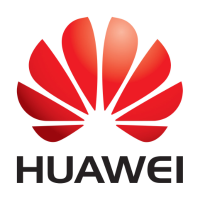
\includegraphics[width=0.25\textwidth]{HUAWEI.png}} % Generic publisher logo
\newcommand*{\ulogo}{
\includegraphics[width=0.25\textwidth]{UHEL.jpg}} % Generic publisher logo


\usepackage{fancyhdr}
\usepackage{lastpage}
\usepackage{url}
\urldef{\mailsa}\path|{mohsin.khan, kimmo.u.jarvinen, valtteri.niemi}@helsinki.fi|
\usepackage[pdfpagelabels,hypertexnames=false,breaklinks=true,bookmarksopen=true,bookmarksopenlevel=2]{hyperref}


%added by the author himself
\usepackage{color}
\usepackage[numbers]{natbib}
\usepackage{calc}
\usepackage{siunitx}
\DeclareSIUnit\mt{\milli\tesla} %% A method for say short cut or new unit!
\sisetup{inter-unit-product = {-}}

\newcommand\ques[1]{``\emph{#1}''}

\setlength\parskip{12pt}
\setlength\parindent{0pt}
\pagestyle{fancy}
\fancyhf{} 
\fancyfoot[C]{\thepage\ / \pageref{LastPage}}
\renewcommand{\headrulewidth}{0pt}



\begin{document}


\mainmatter  % start of an individual contribution

% first the title is needed
%\title{Privacy Protected Subscriber Identification in 5G Network}
%Concealing IMSI in 5G Network Using Identity Based Cryptography

% a short form should be given in case it is too long for the running head
%\titlerunning{Concealing IMSI in 5G Network Using Identity Based Encryption}


\newcommand*{\titleGP}{\begingroup % Create the command for including the title page in the document
\centering % Center all text
\vspace*{\baselineskip} % White space at the top of the page

\rule{\textwidth}{1.6pt}\vspace*{-\baselineskip}\vspace*{2pt} % Thick horizontal line
\rule{\textwidth}{0.4pt}\\[\baselineskip] % Thin horizontal line

{\LARGE Comments on \\[0.3\baselineskip]  5G Security based on the FCC Notice of Inquiry}\\[0.2\baselineskip] % Title

\rule{\textwidth}{0.4pt}\vspace*{-\baselineskip}\vspace{3.2pt} % Thin horizontal line
\rule{\textwidth}{1.6pt}\\[\baselineskip] % Thick horizontal line

\scshape % Small caps
%With minor modifications, this article is also submitted in The 1st EAI International Conference on 5G for Future Wireless Networks  \\[\baselineskip] \par % Location and year

%\vspace*{2\baselineskip} % Whitespace between location/year and editors

{\small Mohsin Khan \\ Kimmo J\"arvinen \\ Valtteri Niemi\par} % Editor list
\ulogo \\[0.3\baselineskip] % Publisher logo
{University of Helsinki \\ Finland\par} 

\vfill % Whitespace between editor names and publisher logo

Published by \\[\baselineskip]
{\small Shield Lab\par} % Editor list
\clogo \\[0.3\baselineskip] % Publisher logo
%{\scshape 2016} \\[0.3\baselineskip] % Year published
{\large Huawei Technologies Co. Ltd.}\par % Publisher

\endgroup}

% the name(s) of the author(s) follow(s) next
%
% NB: Chinese authors should write their first names(s) in front of
% their surnames. This ensures that the names appear correctly in
% the running heads and the author index.
%
\author{Mohsin Khan%
%%\thanks{Please note that the LNICST Editorial assumes that all authors have used
%%the western naming convention, with given names preceding surnames. This determines
%%the structure of the names in the running heads and the author index.}%
\and Valtteri Niemi}  %
%\authorrunning{Lecture Notes of ICST: Authors' Instructions}
% (feature abused for this document to repeat the title also on left hand pages)

% the affiliations are given next
\institute{University of Helsinki, Department of Computer Science,\\
P.O. Box 68 (Gustaf H\"allstr\"omin katu 2b)\\
FI-00014 University of Helsinki\\
Finland\\
\mailsa
%\\
%\url{http://www.springer.com/series/7911}
}

%
% NB: a more complex sample for affiliations and the mapping to the
% corresponding authors can be found in the file "lnicst.dem",
% that is contained in the LNICST LaTeX support package.
%

\toctitle{}
\tocauthor{}
%\maketitle
\titleGP

\thispagestyle{empty}


\section{Introduction}
\label{intro} 

The Federal Communications Commission (FCC), more specifically Public Safety and Homeland Security Bureau (PSHSB) in United States of America (USA) issued a notice of inquiry (NOI) on December 16, 2016. The NOI seeks comments about the security of the future 5G wireless network. In this report we discuss about certain security aspects on which the NOI seeks comments.

The NOI forecasts that 5G is going to be the next evolutionary step in wireless communication and has the potential to be an enormous driver of economic activity. According to the NOI, it is a national priority of USA to foster an environment in which 5G can be developed and deployed across the country. PSHSB considers that they have an opportunity at this stage to ensure that 5G becomes secure by design. Therefore, while FCC is moving quickly to make the spectrum needed for 5G available in the near term, it is also seeking to accelerate the dialogue around the critical importance of the early incorporation of cybersecurity protections in 5G networks, services, and devices.

FCC thinks it is the communication service providers who can best evaluate and address security risks to network operations. Therefore, FCC adopted a rule requiring radio spectrum licensees to submit general statements of their network security plans. This rule is adopted to encourage licensees to consider security in their new 5G networks. PSHSB issued a NOI to seek input on the new issues raised by 5G security to foster dialogue between relevant standards bodies and prospective 5G providers. PSHSB considers that the NOI would complement the important work on cybersecurity that is already taking place within the government and private sector.

The NOI looks holistically at the security implications in the future 5G network. It seeks comments on confidentiality, integrity and availability (CIA) issues. It asks questions about technological primitives used to achieve CIA. These questions span in the area of authentication, encryption, physical security, device security, DoS, DDoS attacks, patch management, and risk segmentation. It also asks fundamental questions about the roles and responsibilities of service providers and device manufacturers. The NOI also seeks comment on the benefit and cost of the security features.

This report tries to comment on certain questions asked in the FCC NOI (DA~16-1282) in the light of 3GPP TR 33.899 document (version 0.6.0, Nov. 2016). The purpose of this report is to provide views and opinions that help in drafting a response to the FCC document's request for comments.

This report focuses particularly on two topics of the FCC inquiry: authentication and encryption (the FCC document's Sections II.A.1 and II.A.2). They are addressed in Sect.~\ref{sec:authentication} and \ref{sec:encryption} of this report, respectively. Some parts of the FCC inquiry (e.g., Sect. II.A.3 ``Physical security'') are not touching the topics of TR 33.899 and they are deliberately left out of the scope of this report. Certain other parts (in particular, the discussion in Section II.B) are relevant, but are addressed within the discussion about authentication and encryption.

\section{Authentication}
\label{sec:authentication}
\subsection{Applicability of Existing Authentication Practices in 5G}
Preserving the confidentiality and integrity of network depends on limiting access to authorized users. Authentication is a pre-requisite of authorization. The NOI seeks comment on the applicability of the existing authentication practices in 5G. It seeks comment \ques{on the use of authentication in networks today and whether existing authentication practices will be applicable to the 5G environment.}

In the existing networks (e.g., UMTS, LTE), authentication scenario is simpler compared to the authentication scenarios in 5G. In the existing networks, a UE trying to connect with the 3GPP network has a subscription of a 3GPP network and has 3GPP credentials. The UE connects to the 3GPP core network (CN) either through a 3GPP defined access network (AN), or through a non-3GPP defined AN (e.g., WiFi, WiMax). UMTS-AKA is used in UMTS to authenticate a UE connecting through a 3GPP defined AN. EAP-AKA is used in UMTS to authenticate a UE connecting through a non-3GPP defined SN. In LTE, EPS-AKA is used. All these protocols authenticate a UE using the 3GPP credentials and create a security context in between a UE and the CN. However, authentication scenarios become more diverse and complex in 5G.

TR 33.899 discusses that existing authentication practices would not readily be applicable in 5G. Because of the complex business model and diversified end-user devices, the authentication requirements become wide and complex. Unlike the legacy networks, the user equipment identifiers are required to be authenticated in 5G. There will be UEs which would not have 3GPP subscription credentials. So, 5G needs authentication mechanism that can authenticate non-3GPP credentials. 

Based on different functionalities, the network will be split into different slices. A network slice can be operated by a 3rd party different from its HN. Authentication is required in between these 3rd parties and UE. UEs will connect through multiple access networks simultaneously. These access networks might be trusted or untrusted non-3GPP access networks, e.g. WiFi, Bluetooth. An authentication framework is required that will consider these scenarios and create a collection of coherent and secure security-contexts.

There will be large number of IoT devices activated almost simultaneously. These bulk activations would create a huge pressure on a central authentication server if such a server's involvement is required in every authentication run. According to 3GPP TR 22.862, the 3GPP system shall support industrial factory deployment where network access security is provided and managed by the factory owner with its ID management, authentication, confidentiality and integrity. The 3GPP system shall support industrial factory deployment where network access security is provided and managed
by the factory owner with its ID management, authentication, confidentiality and integrity. So, requirement of authentication at the edge of the network seems necessary. Like the other legacy networks, the user subscription authentication is also required in 5G. All these concerns are under discussion in TR 33.899, where the contributors are discussing about developing authentication frameworks that would support all the different scenarios. 

It appears that the existing authentication practices will not be sufficient to cater all the new requirements arising in the future 5G network. Existing authentication practices needs to be extended to cater the new requirements and completely new authentication protocol might be needed to solve certain scenarios e.g., authentication at the edge of the network. Potential solutions of authentication framework to cater this diverse need have been proposed based on EPS-AKA, EAP-AKA, EAP-AKA' etc. Non-AKA based solution has also been proposed to authenticate credentials different to existing credentials. The non-AKA based solution uses public-key encryption. Public-key encryption is not used in the legacy networks at all.  

\subsection{Mutual Authentication}
In the NOI published by PSHSB, it seeks comment on \ques{effective use of mutual authentication, in particular, for protecting 5G networks against unauthorized access and end-user devices against attaching to malicious network components, as well as the perceived limitations and drawbacks of those uses}. Mutual authentication is a desirable property in an authentication protocol. In 3GPP networks mutual authentication in between UE and the SN has been incorporated since UMTS and has been strengthened in LTE. As authentication scenarios become diverse and involve many different kinds of entities, 3GPP community needs to be careful about relaxing the requirements of including mutual authentication in an authentication protocol. 

In TR 33.899 different possible solutions are being discussed about the authentication in between the UE and the network. In all the possible solutions mutual authentication has been incorporated. 

In the proposed authentication frameworks in TR 23.799 and TR 33.899 mutual authentication in between UE and network has been incorporated. Binding a serving network public key into the derivation of the radio interface session keys has been proposed to reduce the impact of secret key leakage. Security of RRC idle mode has not been very strong in the legacy networks. In the RRC idle state, UE acquires the system information from the camped cell and uses them to receive paging and obtain other services such as MBMS, D2D, etc. in RRC idle state. When the UE select a cell in RRC idle mode, it does not validate whether the eNB is authentic or fake. As a result, UE may camp to a rogue cell leading to denial of services (such as public safety warnings, incoming emergency calls, real-time application server push services, proximity services, etc.).  It appears that mutual authentication is required to further strengthen the RRC idle mode security.

Subscriber identity privacy is also an important security requirement in 5G. Concealing any long-term  identifier is very central in securing subscription privacy. As found in the discussion in TR 33.899, mutual authentication is instrumental in concealing a long-term identifier. Besides, solutions using mutual authentication have been proposed for relay security, UE's secure access to different network slices and remote credential provisioning.

There has not been any particular discussion in TR 33.899 about any circumstances where mutual authentication would not be beneficial. In some cases, the solution of mutual authentication has been proposed using public key encryption. Apparently the only drawback of mutual authentication would be  increased computational and signalling overhead mostly due to public-key cryptography.

It has been identified that remote credential provisioning of IoT devices is a challenge. Many IoT devices will be resource constrained devices. Embedding enough cryptographic functionality in these devices to enable mutual authentication is challenging. Besides, many IoT devices will try to connect at the same time, which might create a signalling storm.

%\begin{enumerate}
%\item In 3GPP TR 33.899, in Solution 1.11, it discusses about the high level security architecture. Here it proposes that the UE and the network (AUSF) should perform mutual authentication
%\item in 3GPP TR 33.899, in Solution 2.6, it discusses the solution to key issue 2.2 and 3.1. Key issue 2.1 is the impact of the secret key leakage. And key issue 3.1 is the interception of radio interface keys sent between operator entities. To solve these issues, in solution 2.6, it proposes to bind a serving network public key into the derivation of the radio interface session keys. In the detail of the solution it requires mutual authentication in between UE and the network (CP-AU)
%\item In Solution 2.9, it discusses the authentication framework based on EAP. It proposes two alternatives in both of the alternatives it uses mutual authentication in between the UE and the network.
%\item Solution \#2.12, it discusses to solve the following key issues:
%\begin{enumerate}
%\item Authentication framework
%\item AS security during RRC idle mode
%\item Concealing permanent or long-term subscription identifier
%\item Concealing permanent or long-term equipment identifier
%\end{enumerate}
%This solution uses mutual authentication 
%\item Solution \#1.11, it discusses about the high level security architecture.
%\item Solution \#2.9, it discusses the authentication framework based on EAP.
%\item Solution \#2.14 solving key issue 2.5 of Non-AKA based authentication is using mutual authentication
%\item Solution \#2.16: Mutual Authentication between Remote UE and Network over A Relay based on ID-based Credentials
%\item Solution \#2.17: Equipment identifier Authentication using the (IMEI, Device Certificate) binding
%\item Key issue \#3.10: Trusted non-3GPP access
%\item Solution \#3.1: Including a key exchange protocol into the derivation of the radio interface session keys
%\item Solution \#3.3: Security Context Management for UE with Multiple Access Technologies
%\item Solution \#3.7: Algorithms Negotiation Procedure
%\item Solution \#4.1: Network signs selected signalling messages
%\item Solution \#8.2: UE Authentication only by AUSF
%\item Solution \#8.4: UE Authentication by NSI
%\item Solution \#8.7: Security architecture for network slice
%\item Solution \#8.9: Security mechanism differentiation for network slices
%\item Key Issue \#9.1: Mutual authentication of remote UE and network over a relay
%\item Solution \#12.1: Remote credential provisioning – Add Headless IoT device to existing user’s MNO subscription
%\item Solution \#12.3: Secure Mechanism to Achieve Remote Credential Provisioning for IoT devices
%\item Solution \#12.4 Authentication Procedure for credential provisioning
%\end{enumerate}


%\subsubsection{Effective use of mutual authentication to protect 5G Networks Against Unauthorized Access:}
%\subsubsection{Effective use of mutual authentication to protect End-user Device against attaching to malicious network components:}
%\subsubsection{Perceived Limitations and Drawbacks of mutual authentication:}
%\subsubsection{What are the specific considerations applicable to 5G:}
%\subsubsection{Circumstances when mutual authentication is essential:}
%\subsubsection{Circumstances when Mututal Authentication would not be benefical:}
%\subsubsection{Other Authentication Methodologies:}
%\subsubsection{Authentication Challenges in IoT Networks:}
%\subsubsection{Authentication in IoT:}
%\subsubsection{Identity Credentialing and Access Management:}

\section{Encryption}
\label{sec:encryption}

This section discusses several cryptography related issues in TR 33.899 document especially in the light of the FCC inquiry document and its questions. The encryption category of the FCC document is addressed in different parts of TR 33.899. In this section, we focus on the following parts:
\begin{itemize}
\item Security Area~\#1 of TR 33.899 is devoted for architectural aspects. From the encryption point of view, it discusses important high level requirements and constraints for cryptography.
\item Security Area~\#7 of TR 33.899 is devoted for subscriber privacy. The solutions presented in this security area are often based on public-key cryptography and, hence, we discuss it in this section.
\item Security Area~\#17 of TR 33.899 is devoted for cryptographic algorithms. It specifies two key issues: backward compatibility with the cryptographic algorithms of SAE/LTE and quantum safe cryptography. It presents five solutions, all addressing the latter issue. There are no specific solutions presented for the former issue.  
\end{itemize}

As a general note, we state that the cryptographic algorithms that are included in the LTE (i.e., AES, SNOW 3G and Zuc) are still considered cryptographically secure and can be used also in 5G.

\subsection{Public-Key Cryptography}
\label{sec:pkc}

The FCC document (in Para.~12) seeks comments on \ques{the planned deployment and use of encryption to promote 5G security, as well as on the perceived challenges, costs, and benefits of encryption at both the network and device levels}. A significant difference in cryptographic properties that are planned for 5G compared to earlier generations is the inclusion of public-key cryptography. This section provides comments on this topic, especially, in the context of Security Area \#7 ``subscriber privacy''.

Subscriber privacy is an important issue that needs to be protected in 5G. This implies the necessity to conceal information that allows outsiders to identify users. In particular, this means the protection of permanent or long-term subscription identifiers (the IMSI), e.g., from attackers using the so-called IMSI catchers (either passive or active). The privacy requirement may have implications also to the types of encryption used in 5G.

Temporal identifiers and pseudonyms (see Solutions \#7.4, \#7.6, and \#7.12) can protect subscriber privacy in many cases. However, the real identity still needs to be provided, e.g., when the temporal identifier is not available or pseudonyms get unsynchronized. Public-key cryptography enables to transfer the privacy critical identifiers in an encrypted form when the parties (the UE and the network) lack shared secrets. Hence, it offers a good solution to the problem. The disadvantages include significant computational and communication costs. However, combination of temporary identifiers and public-key cryptography can lower this cost significantly because public-key operations are required only when temporary identifiers are not available (see, e.g., Solution \#7.11). Inclusion of public key cryptography also generates new security questions to answer: e.g., how to authenticate or revoke public keys, etc.

TR 33.899 discusses public-key cryptography in many places in its Security Area \#7 (see, e.g., Key Issue \#1.8 and Solutions \#7.2, \#7.8, \#7.9, \#7.11, \#7.14, and \#7.15). In particular they discuss different schemes based on public-key cryptosystems to conceal the IMSI. They include the use of Elliptic Curve Integrated Encryption Scheme (ECIEC) (Solutions \#7.10 and \#7.15), combined with Public-Key Infrastructure (PKI) for authentication of public keys. It is also suggested to use identity-based encryption (Solution~\#7.11) or attribute-based encryption (Solution~\#7.14) to avoid the expense of using PKI for authentication of public keys. We estimate that the solutions based on public-key cryptography, when combined with pseudonyms, are the most feasible solutions to achieve high level subscriber privacy. TR~33.899 discusses the use of public-key cryptography also in Security Area \#2 ``authentication''. There it is used, in particular, for enabling authentication locally at the edge of the network by using identity-based public-key cryptography (see Key Issue \#2.5 and Solution \#2.14).

% Requires PKC:

% Key Issue~\#1.8 UEs with asymmetric keys

% Solution~\#7.2 proposes to use public-key encryption with a network's public-key for sending the IMSI. Solution~\#7.3 is essentially the same thing with more details. Solution~\#7.7 addresses the legal interception problems of Solution~\#7.3.

% Solution~\#7.8 suggest an opportunistic encryption procedure where public-key encryption is used for IMSI in the case identification with temporary identity fails. Usually opportunistic encryption means that one tries to use encryption always but removes encryption if this is not possible. Here it means something different: use public-key cryptography if the procedure with temporary identifiers fails. The solution also has some vulnerabilities against the man-in-the-middle attacks so it is unclear how useful it is.

% Solution~\#7.9 proposes to use Diffie-Hellman key exchange to thwart passive attackers because public-keys are not authenticated (as far as we can tell). The motivation for such a countermeasure is questionable because it is still relatively expensive (requires public-key cryptography). Solution~\#7.10 proposes a similar scheme, but this time with Diffie-Hellman Integrated Encryption Scheme such as Elliptic Curve Integrated Encryption Scheme (ECIEC) and authenticated public keys via Public-Key Infrastructure (PKI). The solution is more expensive but thwarts also active attackers.

% Solution~\#7.11 proposes to use identity based public-key encryption for protecting identity. This avoids the problem of authenticating the public keys.

% Solution~\#7.14 suggests using attribute-based encryption to protect IMSI. This is used only when the temporary identifier is not available. 

% Solution~\#7.15 proposes to use ECIES to encrypt the IMSI. How is this different to Solution~\#7.10?

% No PKC needed:

% Solution~\#7.4 proposes a privacy enhanced IMSI which is a short-lived identifier. The idea is conceptually close to pseudonyms.

% Solution~\#7.5 suggests using randomness from channel estimation to generate short-term identifiers. Perhaps such randomness could be used as a part of seeding a pseudo-random number generator (PRNG) but it is unclear why a PRNG is not a sufficient solution.

% Solution~\#7.6 discusses parameters for refreshing the temporal identifier, i.e., when the identifier needs to be updated.

% Solution~\#7.12 proposes using pseudonyms (temporal IMSI shared between the UE and the home network) to conceal subscriber's identity. This offers a low cost solution to the subscriber privacy problem because public-key cryptography is not needed.

% Solution~\#7.13 proposes to refresh core network short-term identifiers.

% Solution~\#7.16 shows a mechanism for assigning temporary identifiers so that the network generates them but the UE checks that it is truly new.

To address the FCC documents request for comments, we conclude that \ques{the planned deployment and use of encryption} (see Para.~12), and public-key encryption in particular, significantly strengthens the cryptographic toolkit available for improving security features of 5G compared to previous generations. Public-key cryptography allows more flexible and scalable ways to \ques{address encryption key management and distribution mechanisms} (in Para.~13). We assess that securing the envisioned 5G network of heterogeneous devices would be difficult without public-key cryptography so the decision to include public-key cryptography is justifiable. However, this does not come for free because all forms of public-key cryptography are significantly more costly than the symmetric encryption schemes. This can be a problem for \ques{a 5G environment in which innumerable, low-cost devices are expected to operate} (in Para.~13) because the hardware-related resources for some of such devices can be expected to be very limited. This holds particularly for the IoT scenario included in 5G.

The above discussion is relevant also for the question in Para.~13, where the FCC document asks: \ques{whether currently available encryption protocols are effective in securing devices and are like to be effective in a 5G environment}. We can conclude that the answer  is `no' because many of the additional security features require public-key cryptography and, hence, support for it needs to be added to 5G. However, it is noteworthy that Security Area~\#17 about cryptographic algorithms does not mention any specific public-key cryptography algorithms to be used in 5G. It only discusses the quantum safe algorithms (see Sect.~\ref{sec:qsc}), but without a doubt also traditional public-key algorithms need to be included. Because of performance, key lengths and ciphertext sizes, elliptic curve cryptosystems would be the most appropriate candidates.

\subsection{Low Latency Encryption}
\label{sec:latency}

5G is required to offer superior performance compared to previous generations of mobile communication and one side in this requirement is to offer communication with very low latency. In multiple places, TR 33.899 mentions that the latency requirements range from $<$1\,ms to $<$10\,ms. It is not completely clear based on TR 33.899 what this latency is expected to include, does it affect both the control and user plane, etc. Nevertheless, these requirements for low latency have many connotations to security and encryption. Many of questions asked in the FCC document also relate to the requirement for low latency: in particular, the questions about \ques{the perceived challenges, cost, and benefits of encryption} (in Para.~12), \ques{whether currently available encryption protocols are effective in securing devices and are likely to be effective in a 5G environment in which innumerable, low-cost devices are expected to operate} (in Para.~13), and \ques{whether encryption is necessary for all 5G communications} (in Para.~14). 

As a general note, we state that the low latency requirement appears to be very hard to address securely. Already the speed of light mandates that all parties involved in the communication must be in close geographical locations: latency of 10\,ms translates to approximately 1500\,km round-trip at the speed of light. For instance, the latency requirement means that it is impossible to communicate with the home network if it is some thousands of kilometers away. Hence, the only way seems to be to reduce the role of the home network or otherwise tolerate longer latencies (at least for the control plane). Another aspect is the latency of cryptographic operations. This affects, in particular, the use of public-key cryptography because secure public-key algorithms are computationally complicated and often latencies of $<$1\,ms can be achieved only with powerful processors and/or with the help of hardware accelerators. 

The above discussion about reducing the role of the home network is relevant for the FCC document's request for comments (in Para.~14): \ques{We seek comment on whether the decisions made by the 3GPP standards body that resulted in non-encryption for such systems are rooted in increased latency, degraded performance due to added signaling or computational requirements, and interest in minimizing changes to LTE standards as 5G is standardized, or other factors. We inquire about what lessons, if any, can be learned from the underlying rationale of these decisions as they pertain to encryption for 5G communications.}. We see that there is a risk to create security vulnerabilities if latency is too much prioritized over security. Hence, it is essential to verify that any decisions made to decrease latency do not lead to security vulnerabilities that, e.g., allow \ques{tracking the movements of individuals}.

TR 33.899 discusses the effects of the requirement for low latency in several places and, especially, in Security Area~\#1. We summarize the discussion next. 
Key Issue~\#1.13 discusses the challenges created by low latency requirements, which  may prevent using strong security mechanisms and lead to severe vulnerabilities. It concludes that at least the control plane should be fully secured even if this leads to longer latency. 
Solution~\#1.12 claims a solution to the latency problem by using Forward Error Correction (FEC) codes, but it provides very little details and we estimate that it does not provide sufficient cryptographic security if more attention would be given to it. 
Solution~\#1.15 suggest to use AES as a fast stream cipher, namely use it in CTR (counter) mode, for low latency. Actually this solution is already in use in LTE.
%We think this can be a viable solution as hardware support for AES(-CTR) is often available and can be very efficient for encrypting several blocks because the CTR mode can process blocks in a pipelined manner. %However, pipelining does not give latency improvements for small amounts of data. 
It would also be possible to extend AES-CTR to AES-GCM (Galois/Counter mode) which would provide confidentiality, integrity and authenticity with little extra overhead compared to AES(-CTR) (see Sect.~\ref{sec:ae}).
Solution~\#1.18 proposes that the control plane is allowed to have longer latency than the user plane. This seems reasonable as it would allow more elaborated security measures to be used for control plane including public-key cryptography. The security of the user plane could be ensured on higher communication layers (transport and application layers). % , which are not affected by the latency requirements. 
%However, even this solution may lower security to some extent because it requires storing old security associations in the roaming network as pointed out by Solution~\#1.18.
The message of TR 33.899 seems to be that the requirements for low latency should affect only the user plane. Despite this, reducing the latency of the control plane is still important and discussed in TR 33.899 (e.g., Solutions \#1.16 and \#1.17).
%The latency of the control plane could be reduced by using an intermediate key in the roaming network (that is still negotiated when first connecting to the network and refreshed every once and while) as suggested in Solution~\#1.16 ``data efficient re-keying''. Another solution Solution~\#1-17 proposes to delegate some of the functionalities of the home network to the serving network via a delegated subscriber server (DSS) so that the long-term subscriber secret key is not given to the DSS. However, these techniques have certain security shortcomings and may enable frauds from the visiting network as pointed out in the solutions.

Recent advances in cryptography may help in reducing the latency. E.g., using authenticated encryption instead of a cipher and a MAC leads to shorter latency (see Sect.~\ref{sec:ae}). Also some ciphers that are designed to minimize latency have been proposed during the recent years (e.g., PRINCE\footnote{Published in the article: Julia Borghoff, Anne Canteaut, Tim Güneysu, Elif Bilge Kavun, Miroslav Knezevic, Lars R. Knudsen, Gregor Leander, Ventzislav Nikov, Christof Paar, Christian Rechberger, Peter Rombouts, Søren S. Thomsen, Tolga Yalçın: ``PRINCE --- A Low-Latency Block Cipher for Pervasive Computing Applications'', ASIACRYPT 2012, LNCS 7658, pp. 208-225, 2012.}) and they could later improve the situation. The downside is that, to the best of the authors' knowledge, low latency ciphers have not been standardized so far and still lack the level of public scrutiny expected from secure cryptography.

The above discussion is relevant in the light of the FCC document's question (in Para. 14): \ques{whether encryption is necessary for all 5G communication}. Including encryption to all 5G communication would benefit security, but the requirements for low latency seem to be contradicting with this. Hence, the most reasonable answer to the question appears to be that although using encryption for all communication would be good from the security point of view, it is maybe not possible to achieve all requirements if everything is encrypted. At least the control plane must be fully encrypted, but the use of encryption on the user plane can possibly be left for higher abstraction layers. In addition to the above question, this answers also to the following questions (in Para. 15): \ques{whether 5G service providers should distinguish between the application of encryption to products that would operate on the 5G control plane and those that would be part of the user plane?} and \ques{how should such a distinction be made?}.

\subsection{Quantum Safe Cryptography}
\label{sec:qsc}

The FCC document seeks comments (in Para.~12) on \ques{the planned deployment and use of encryption to promote 5G security, as well as on the perceived challenges, costs, and benefits of encryption at both the network and device levels}. As already discussed in Sect.~\ref{sec:pkc}, 5G is expected to include public-key cryptography (see Sect.~\ref{sec:pkc}). The current public-key cryptosystems (e.g., RSA, ECDH and ECDSA) are not enough to secure devices if the attackers would be able to utilize large-scale quantum computers in their attacks because they are vulnerable to Shor's algorithm. %The emerge of large-scale quantum computers would make current public-key cryptosystems (e.g., RSA, ECDH and ECDSA) obsolete. 
Secret-key cryptography is believed to be less affected and security level can be retained to the original level by doubling the key size (e.g., use AES-256 instead of AES-128). Although the FCC inquiry does not directly mention quantum safe cryptography, we think it is relevant in the light of the questions asked in Section II.A.2 and, especially, the above request of comments.

TR 33.899 acknowledges the need for quantum safe cryptography in 5G (in Key Issue~\#17.2). We agree that it is important to address the quantum threat in the 5G specifications because the 5G network can be expected to be used for a long time (several decades). Hence, it is possible that large-scale quantum computers will be built in that time frame making the current public-key cryptography vulnerable. The problem is that the field of quantum safe cryptography is not matured yet and there are no clear alternative for the current public-key cryptosystems. Instead, there are multiple proposals which have not been fully analyzed in terms of security (both classical and quantum) or efficiency. TR 33.899 provides five possible solutions to the quantum threat and the problem of not having a clear replacement algorithm.

Solution~\#17.1 suggests to incorporate a quantum safe algorithm ``from day one''. It is very unlikely that a well established and standardized algorithm exists when 5G specifications are fixed. Solution~\#17.1 acknowledges this problem and suggest to delay the selection as late as possible. However, selecting a quantum safe algorithm even at that point can be very problematic because 5G specifications will be fixed in the near future. NIST of the USA has initiated a process for selecting a portfolio of quantum safe algorithms followed later by standard(s), but this process is not expected to finish before 2020s. There are many alternative solutions for quantum safe cryptography available, but none of them has received the public scrutiny that is expected from secure cryptosystems. Hence, fixing an algorithm in the near future is risky. There is a risk of wasting a lot of resources in implementing cryptosystems that are never being used because (a) progress in quantum computing research does not advance, (b) the selected algorithm is not secure (if broken in the coming years), (c) other more secure or efficient alternatives are developed, and/or (d) the parameters of a standardized version of the algorithm may be different from the selected one even if the same cryptographic technique is selected for the future standards and 5G specification. Especially (b) is critical because having insecure cryptosystems in the 5G portfolio could lead to severe security issues. Based on all this, we feel that it may not be possible to select a quantum safe algorithm for 5G ``from day one''.

TR 33.899 proposes two solutions that do not require fixing the algorithm in the 5G specifications: Solution~\#17.3 allows the home network to update algorithms in the UE and Solution~\#17.4 allows secure negotiation of algorithms when support for an algorithm is already available in the UE and the home network\footnote{ßSolution~\#17.5 is similar to Solution~\#17.4, but allows the UE and the serving network to securely negotiate an algorithm.}. The former allows the home network to update the public-key algorithms to quantum safe algorithms when such algorithms become standardized and/or when the quantum threat becomes a more urgent matter. The downside is that this would be a software update which may lead to inefficient and insecure (against side-channel attacks) cryptographic implementations. The latter allows the use of quantum safe algorithms when both the UE and the home network have support for them. This does not have the drawback of the former solution because vendor optimized implementations (including hardware support) is permitted, but this solution does not permit rapid updates of the algorithms or updating old devices. We feel that either of these solutions or, preferably, a combination of them are more feasible options for mitigating the quantum threat in 5G.

TR 33.899 proposes message flexibility in a solution Solution~\#17.2 to support larger signature and public-key sizes that are needed for most quantum safe algorithms. It allows easier integration of algorithms in the future and makes sure that no alternative needs to be ruled out because of such issues. However, we note that there are quantum safe proposals (namely, ones based on supersingular isogenies) which have smallish key sizes (roughly comparable to the RSA), although TR 33.899 hints that all quantum safe proposals involve significantly larger keys.

To summarize, we agree that it is important to address the quantum threat in the 5G specifications although established replacement algorithms will not be available at the moment. The solutions enabling algorithm updates and use of other supported algorithms should provide enough means to address the problem in the future. It would also be good to have a solution to force the use of quantum safe algorithms instead of the existing public-key algorithms in the future. That is, a solution to remove algorithms which are no longer considered secure.


\subsection{Authenticated Encryption}
\label{sec:ae}

As discussed in Sect.~\ref{sec:latency}, the requirement for low latency sets strict constraints on security and encryption. The 5G environment is also expected to include very resource constrained devices which brings new challenges for implementing encryption. These challenges are relevant for the FCC document's request for comments on \ques{whether currently available encryption protocols [...] are likely to be effective in a 5G environment in which innumerable, low-cost devices are expected to operate}  (in Para.~13) and \ques{on the perceived challenges, costs, and benefits of encryption at both the network and device levels} (in Para.~12). 

The basic features expected to be achieved with the use of encryption are confidentiality, integrity, and authenticity. Traditionally, the first is achieved with a cipher (e.g., the AES block cipher with an appropriate mode of operation) whereas the latter two are achieved with a separate message authentication code (e.g., HMAC based on cryptographic hash functions). Hence, achieving all three features requires both encryption and MAC to be computed with the data, which can be expensive. 

Authenticated encryption refers to modes of operations which allow to use a block cipher so that all three features are achieved at once, leading to significant efficiency and usability benefits. The most well known authenticated encryption scheme is AES-GCM (Galois/Counter Mode), but many alternatives are available, some of which are more efficient. Authenticated encryption is already included in several standards: e.g., NIST Special Publication 800-38D (for GCM) and ISO/IEC 19772:2009. There is also an on-going cryptographic competition on authenticated encryption, the so-called CAESAR competition\footnote{See \url{http://competitions.cr.yp.to/caesar.html}.}. 

TR 33.899 includes discussion about which parts of the communication should be protected for confidentiality and integrity (the latter appears to imply also authenticity) in Key Issues~\#1.9--12. However, TR 33.899 seems to have completely missed the possibility of using authenticated encryption. Using authenticated encryption could give valuable advantages, e.g., in the context of low latency requirements (see Sect.~\ref{sec:latency}) and low implementation footprint (for small devices) because only one cryptographic primitive would be needed.


\section{Conclusion}
\label{sec:conclusion}

In this report, we have provided some insight on 5G security based on the FCC inquiry document especially on the topics of authentication and encryption. %We conclude that the planned security features of the future 5G require significant chan. 
We did not find any specific areas discussed in the FCC document which have been completely neglected in TR 33.899, at least in the context of authentication and encryption. However, because the process for 5G specifications is still unfinished, we find that certain solutions are not yet complete or fully mature and further work is required to validate their feasibility and security and to choose the most appropriate solutions from the many competing alternatives available in TR 33.899. Additionally, specific public-key cryptosystems need to be discussed in Security Area \#17 if they are to be included in 5G specifications so that their security, efficiency and general suitability can be evaluated. 



%\subsection{Lightweight Cryptography for the IoT Applications}
%\label{sec:iot}

%The FCC document asks comments about the necessity of encryption for all communication and, in particular, whether 



%\begin{thebibliography}{4}

%\end{thebibliography}

\end{document}
